\documentclass[aps,pre,twocolumn,showpacs,amsmath,amssymb]{revtex4-1}

\usepackage{graphicx}
\usepackage{color}

\usepackage[portuguese]{babel}
\usepackage[utf8]{inputenc}
\usepackage[T1]{fontenc}

\usepackage{titlesec}

\setlength{\belowcaptionskip}{0pt}

\titlespacing*{\section}{0pt}{\baselineskip}{\baselineskip}
\titlespacing*{\subsection}{0pt}{\baselineskip}{\baselineskip}

\hfuzz 1pt
\vfuzz 1pt

\setlength{\parskip}{\baselineskip}

\begin{document}

\title{Exercício 07: Equações diferenciais ordinárias}

\author{Ernesto González, Inês Rebanda, Rafael Lopes}

\begin{abstract}
  Utilização e análise dos métodos de Euler e de Runge-Kutta de $4^{a}$ ordem para a resolução de EDOs. Comparação entre diferentes passos de integração e soluções analíticas. Estudo do decaímento radioativo, epidemia de zombies e lançamento oblíquo de um projétil.
\end{abstract}

\maketitle

\section{Decaímento radioativo}
O decaimento radioativo do Polónio-201 é dado pela equação $\dot{N}(t)=-kN(t)$ onde N(t) é a densidade de núcleos radioativos no instante $t$ e $k$ é a taxa de decaimento dada por $k=2.3 horas^{-1}$. Sendo $N(0)=1$ implementamos o método de Euler e o de Runge-Kutta de $4^{a}$ ordem.

\begin{figure}[h]
   \begin{center}
    \includegraphics[width=\columnwidth]{71a.png} \\
\caption{Gráfico do decaimento radioativo definido por $\dot{N}(t)=-kN(t)$ e $N(0)=1$, calculado pelo método de Euler para passos de integração $h=\{0.5,0.7,1\}$ e gráfico da solução analítica $N(t)=e^{-2.3t}$.}
  \label{fig.exemplo}
   \end{center}
  \end{figure}

Primeiramente implementou se o método de Euler e traçou-se o gráfico para a solução numérica de N(t) com passos de integração $h=\{0.5, 0.7, 1\}$. Comparamos também com a solução analítica $N(t)=e^{-2.3t}$.
Para $h=0.5$ o gráfico converge rapidamente para a solução e a suas oscilações são ligeiras sendo especialmente pequenas após $t=1$.
Para $h=0.7$ o gráfico também converge rapidamente para a solução mas não tão rápido como $h=0.5$ e as suas oscilações são também de maior amplitude.
Para $h=1$ o comportamento do gráfico muda e em vez de convergir ele diverge aumentando a cada iteração a amplitude das oscilações. Isto acontece pois enquanto que com $h=0.5$ e $h=0.7$ ao efetuar a equação $\dot{N}(t)=-kN(t)$ o resultado é menor que 1 (que é o resultado inicial), em $h=1$ o resultado vai ser maior que 1, em módulo, fazendo com que divirja. \\


Seguidamente utilizou-se o método de Runge-Kutta de $4^{a}$ ordem e traçou-se o gráfico do seu desvio e do de Euler ao valor analítico em $t=5\, horas$ em função do tamanho do passo (em escala log-log), com passos $h=\{1,\frac{1}{2},\frac{1}{4},\frac{1}{8},\frac{1}{16},\frac{1}{32},\frac{1}{64}\}$.

\begin{figure}[h]
   \begin{center}
    \includegraphics[width=\columnwidth]{71b.png} \\
\caption{Desvio, $d$, dos valores $N(t=5)$ econtrados para as soluções do PVI $\dot{N}(t)=-kN(t)$ e $N(0)=1$, calculadas numericamente pelos métodos de Euler e Runge-Kutta de $4^{a}$ ordem, em função do passo de integração usado no método. Os passos usados foram $h=\{1,\frac{1}{2},\frac{1}{4},\frac{1}{8},\frac{1}{16},\frac{1}{32},\frac{1}{64}\}$.}
  \label{fig.exemplo}
   \end{center}
  \end{figure}

Pelo gráfico vê se que o método de Runge-Kutta de $4^{a}$ ordem tem sempre um erro inferior ou igual, para o mesmo valor de $h$, do que o método de Euler. Por isso neste caso é o método mais eficaz dos dois.\\
O declive das linhas dão-nos a ordem de convergência do respetivo método, isto é, o expoente pelo qual o desvio, $d$ varia com o passo de integração $h$. Para o método de Euler, em $h\in [\frac{1}{64},\frac{1}{2}]$ a ordem de convergência é, aproximadamente $O(h^{0.5})$. Já em $h\in [\frac{1}{2},1]$ é $O(h^{18})$. Para o método de Runge-Kutta de ordem 4, em $h\in [\frac{1}{64},\frac{1}{2}]$ a ordem de convergência é, aproximadamente $O(h^{-0.74})$ e em $h\in [\frac{1}{2},1]$ é $O(h^{19.5})$.

\section{Epidemia de zombies}
Considere-se o cenário de uma epidemia de zombies. Sabe-se que um zombie contagia um humano com taxa $c$, um humano mata um zombie com taxa $a$ e um zombie mata um humano com taxa $b$. Assim, as equações da população de humanos, $H$, e de zombies, $Z$ são
\begin{equation}
\begin{split}
    \frac{dH}{dt} &= -(b+c)HZ \\
    \frac{dZ}{dt} &= (c-a)HZ
\end{split}
\end{equation}
Nas Figuras 3 e 4 encontram-se os resultados das simulações para $a=0.05$, $b=0.06$, $c=0.02$ usando o método de Euler e $a=0.01$, $b=0.03$, $c=0.04$ usando o método Runge-Kutta de ordem 4, partindo de várias populações iniciais.

\begin{figure}[hbt!]
   \begin{center}
    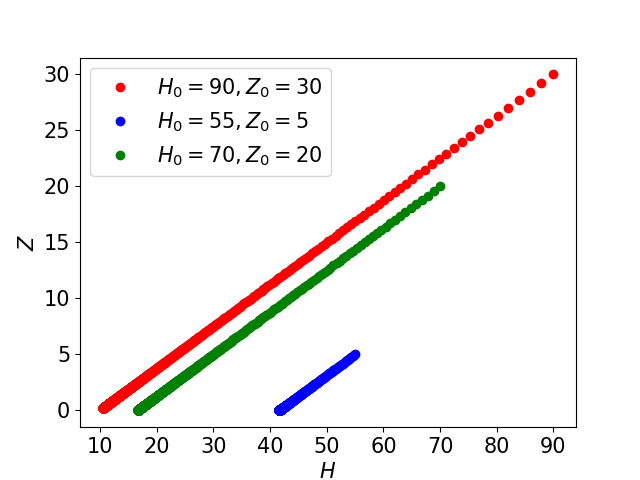
\includegraphics[width=\columnwidth]{epidemiazombieeuler.png} \\
\caption{Resultados da simulação da epidemia de zombies descrita por     $\dot H=-(b+c)HZ\; \wedge \;\dot Z=(c-a)HZ$ usando o método de Euler para $a=0.05$, $b=0.06$, $c=0.02$ e diferentes pares $H_0$, $Z_0$.}
  \label{epidemiaeuler}
   \end{center}
  \end{figure}

\begin{figure}[hbt!]
   \begin{center}
    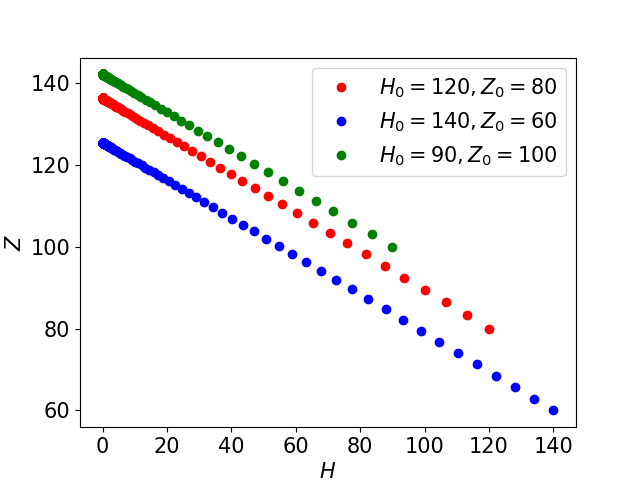
\includegraphics[width=\columnwidth]{epidemiazombierk.png} \\
\caption{Resultados da simulação da epidemia de zombies descrita por     $\dot H=-(b+c)HZ\; \wedge \;\dot Z=(c-a)HZ$ usando o método de Runge-Kutta para $a=0.01$, $b=0.03$, $c=0.04$ e diferentes pares $H_0$, $Z_0$.}
  \label{epidemiark}
   \end{center}
  \end{figure}
Nos três casos analisados na Figura 3, a população de zombies, $Z$, ficou extinta. Já nos casos expostos na Figura 4, a população de humanos, $H$, ficou extinta.\\
Estudemos o sistema (1). Se $c-a>0$, então a taxa a que os zombies contagiam humanos, $c$, é maior do que a taxa a que os humanos matam zombies, $a$. Neste caso, os humanos são extintos.\\ Se a taxa a que os humanos matam zombies, $a$, for maior do que a taxa a que os zombies contagiam humanos, $c$, temos $c-a<0$. Neste caso o destino do sistema será definido pelas condições iniciais e pelas taxas de crescimento das populações. Vejamos com mais atenção este caso.
Definindo $\alpha =b+c$ como a taxa total de destruição de humanos e $\beta = c-a$ a taxa de criação de zombies, reescrevemos o sistema (1) como
\begin{equation}
    \frac{d(\beta H+\alpha Z)}{dt}=-\beta \alpha HZ + \alpha \beta HZ =0,
\end{equation}
pelo que $\beta H + \alpha Z$ é constante. Se a população de zombies for extinta, então a população final de zombies é nula: $Z_f=0$. Assim, do facto de $\beta H + \alpha Z$ ser constante vem
\begin{equation}
    -\beta H_f= -\beta H_0 - \alpha Z_0
\end{equation}
Logo para que os humanos tenham sobrevivido vem
\begin{equation}
\begin{split}
   -\beta H_f>0 &\iff -\beta H_0 - \alpha Z_0 >0 \\
   &\iff -\beta H_0 > \alpha Z_0
\end{split}
\end{equation}

\section{Lançamento oblíquo}
Considere-se um lançamento oblíquo de um projétil. As equações do movimento são:
\begin{equation}
\begin{cases}
    \dot{x}=0\\
    \dot{y}=-g\\
    \dot x(t)=\dot v_x(t)\\
    \dot y(t)=\dot v_y(t)
\end{cases}
\end{equation}
\\
em que $g$ é o módulo da aceleração da gravidade, e a velocidade $v_0=20\,ms^{-1}$ faz um ângulo de $\pi /4$ com a horizontal.
Na Figura 5, encontra-se a trajetória seguida pelo projétil calculada numericamente pelos métodos de Euler e Runge-Kutta, bem como a solução analítica do sistema, partindo de $x_0=0$ e $y_0=0$.
\begin{figure}[hbt!]
   \begin{center}
    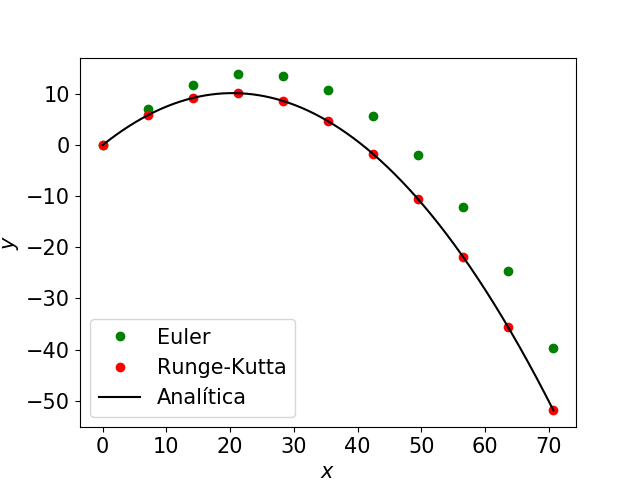
\includegraphics[width=\columnwidth]{trajetoriaprojetil.png} \\
\caption{Trajetória do projétil cujo movimento é dado por $       \dot v_x(t)&=0\wedge \dot v_y(t)&= -g\wedge x(t)&=v_x(t)\wedge y(t)&= v_y(t)$, calculado numericamente com os métodos de Euler e Runge-Kutta de ordem 4 e analiticamente com $x=x_0+v_0t \wedge y=y_0+v_yt-0.5gt^2$, para valores iniciais $x_0=0$, $y_0=0$, $v_{x_0}=20cos(\frac{\pi}{4})$ e $v_{y_0}=20sin(\frac{\pi}{4})$.}
  \label{trajetoriaprojetil}
   \end{center}
  \end{figure}
Na Tabela I encontram-se os valores de $y(t=5)$ para os diferentes métodos utilizados.

\begin{table}[hbt!]
\centering
\caption{Valores de $y$ quando $t=5\,s$ para os métodos de Euler e Runge-Kutta de ordem 4 e da solução analítica para o sistema $       \dot v_x(t)&=0\wedge \dot v_y(t)&= -g\wedge x(t)&=v_x(t)\wedge y(t)&= v_y(t)$, partindo de $x_0=0$, $y_0=0$, $v_{x_0}=20cos(\frac{\pi}{4})$ e $v_{y_0}=20sin(\frac{\pi}{4})$.}
\begin{tabular}{|c|c|}
    \hline
Método & y(t=5)      \\ \hline
Euler & -39.65182188134526  \\ \hline
Runge-Kutta & -51.91432188134523  \\ \hline \hline
Analítica &  -51.914321881345415\\ \hline
\end{tabular}
\end{table}
\\
Na Figura 5, pode ser observado a representação da trajétoria de y(x) calculada para cada Método, e ainda pode ser observada a curva da trjetória real, obtida analiticamente. Ao observar a curva obtida atravês do Método de Runge-Kutta de 4ª ordem podemos verificar que esta curva coicide com a curva analitíca.
Podemos então inferir que isto dá-se pois o seu erro estará associado À 4ª ordem de t, o que significaria que os valores de x e y analíticos serão sempre idênticos aos obtidos com o Método Runge-Kutta de 4ª ordem, pois as funções x e y são funções de t de 2ª ordem.
\\
A partir da Figura 5 pode ser também inferido que a trajetória obtida através dos valores do método de Euler começa a divergir da curva analítia apresentando um desvio cada vez maior. Então, podemos concluir que o Método de Euler tem uma precisão inferior ao Método de Runge-Kutta de 4ª ordem.
Sendo que esta conclusão é também corruburada pelos valores da Tabela I.
\\
\\
Consideremos agora que o projétil está sujeito à resistência do ar, em que a aceleração tem um termo adicional de $\gamma v^2$ na mesma direção da velocidade, mas sentido contrário. As equações do movimento passam a
\begin{equation}
    \begin{split}
        \dot v_x(t)&=-\gamma v_x^2(t)\\
        \dot v_y(t)&= -g + \gamma v_y^2(t),\quad \text{se}\; v_y(t)<0 \\
        \dot v_y(t)&= -g - \gamma v_y^2(t),\quad \text{se}\; v_y(t)\geqslant0 \\
       \dot x(t)&=v_x(t) \\
       \dot y(t)&= v_y(t)
    \end{split}
\end{equation}
Na Figura X, encontra-se a trajetória do projétil encontrada pelos métodos de Euler e Runge-Kutta de ordem 4.
\begin{figure}[hbt!]
   \begin{center}
    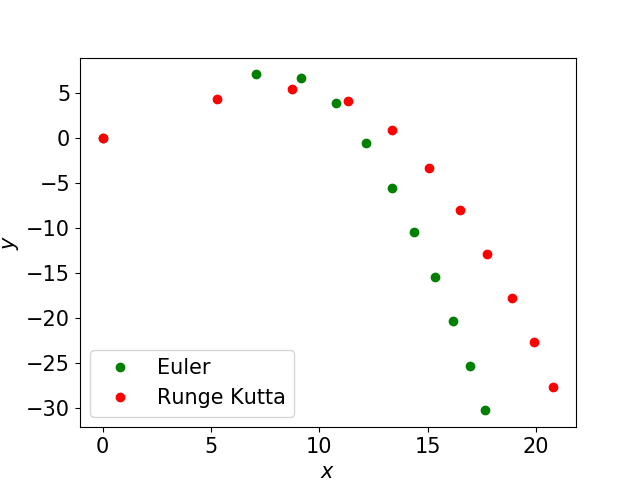
\includegraphics[width=\columnwidth]{trajetoriaprojetildissipativo.png} \\
\caption{Trajetória do projétil cujo movimento é dado por $               \dot v_x(t)=-\gamma v_x^2(t) \wedge
        \dot v_y(t)= -g + \gamma v_y^2(t),\quad \text{se}\; v_y(t)<0\wedge
        \dot v_y(t)= -g - \gamma v_y^2(t),\quad \text{se}\; v_y(t)\geqslant0\wedge
        x(t)&=v_x(t)\wedge y(t)&= v_y(t)$, calculado numericamente com os métodos de Euler e Runge-Kutta de ordem 4, para valores iniciais $x_0=0$, $y_0=0$, $v_{x_0}=20cos(\frac{\pi}{4})$ e $v_{y_0}=20sin(\frac{\pi}{4})$.}
  \label{trajetoriaprojetildissipativo}
   \end{center}
  \end{figure}
Resolvendo analiticamente (6), para as condições iniciais $x_0=0$, $y_0=0$, $v_{x_0}=20cos(\frac{\pi}{4})$ e $v_{y_0}=20sin(\frac{\pi}{4})$, obtemos
\begin{equation}
    \begin{split}
        v = \frac{1}{\gamma t+20cos(\frac{\pi}{4})}\\
        y =
    \end{split}
\end{equation}
\end{document}
